\chapter{Intra-Vehicles}

\section{ISO/OSI Layers}
In telecommunication the idea is to divide each steps into layers starting from the application layer to the fisical ones, every layers have different function and it needs different protocols. Each layer can interact with the one that is above or below it and the communication of two layers follow rigid and specifics rules. Nowadays the standard \textit{de iure} is the \textbf{ISO/OSI}, instead the the \textit{de facto} standard is the \textbf{TCP/IP} that relax the rigid guidelines. The \textit{ISO/OSI} has seven layers (bottom to top):
\begin{enumerate}[nosep]
    \item \textbf{physical layer}: specifies the mechanical and electrical properties to transmit bit (in the ``real'' world) and to control time synchronization.
    \item \textbf{data link layer}: checked the transmission of the frame, error checking, frame synchronization and flow control.
    \item \textbf{network layer}: it is used for the transmission of the packets, it is also know as \textit{IP Layer}, in is normally use in ethernet.
    \item \textbf{transport layer}: reliable end to end transport segment, you can manage how the data have to flow. In 99.99 \% of the car domain it doesn't need.
    \item \textbf{session layer}: establish and tear down sessions.
    \item \textbf{presentation layer}: define the syntax and the semantics of information.
    \item \textbf{application layer}: uses data transmitted via physical medium.
\end{enumerate}
In the first module we need only two layers: \textbf{physical layer} and \textbf{data link layer}. We have to study the behaviour of the communication protocols like CANBus, LIN, FlexRay, MOST and Ethernet in this two layers. Starting from the \textbf{transmission medium}, normally the hardware pieces that we use to interact with is:
\begin{itemize}[nosep]
    \item \textbf{transceiver}: is used to ``convert'' analog signal to bits (brain less).
    \item \textbf{controller}: control the communication (brain full).
\end{itemize}
Initially the idea is to focus a little more on \textbf{CANBus}, the \textbf{\textit{Physical Layer}}: is compose by three component: \textbf{Physical Signaling - PLS}, \textbf{Physical Medium Attachment - PMA} and \textbf{Media Dependant Interface - MDI}.
\begin{enumerate}[nosep]
    \item \textbf{physical signaling}: the main purpose is to understand the bit encoding/decoding (if it is \textit{NRZ} or \textit{Manchester}) and to mantein the synchronization all over the network, every transceiver it must have a the same clock source. The synchronization is the most important things both for the bit encoding/decoding and for don't introduce delay in the communication.
    \item \textbf{physical medium attachment}: driver/receiver characteristics based on the communication protocol.
    \item \textbf{media dependant interface}: the connector for access to the physical medium.
\end{enumerate}
\textbf{\textit{Data Link Layer}} is compose by two component: \textbf{Logical Link Control - LLC} and \textbf{Medium Access Control - MAC}.
\begin{enumerate}[nosep]
    \item \textbf{logical link control}: from now on, we start to call \textit{frame} the data that are send/receiver from the physical channel. It is used for \textit{acceptance filtering} that permit to decide if a frame is important for the application above the \textit{controller} and if not discard it. This component include also the \textit{overload notification} and \textit{recovery management} in the case there is an error on the communication they could ask to a re-transmit the data.
    \item \textbf{medium access control}: is purpose is \textbf{error detection} it could check the data encapsulation/decapsulation, frame coding and error detection/signaling/handling.
\end{enumerate}

\section{Network Topology - The Bus System}
\begin{figure}[h]
    \centering
    \begin{minipage}[t]{0.3\textwidth}
        \centering
        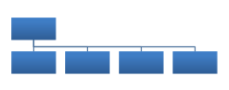
\includegraphics[width=\textwidth]{img/line}
        \caption{\textit{Line Topology}}
        
        \begin{flushleft}
            In the \textbf{Line} topology also know like \textbf{\textit{Bus}} topology each node is connected by interface connectors to a single center cable. It is cheaper than the others and it has lower complexity but it is not very robust.
        \end{flushleft}

    \end{minipage}
    \begin{minipage}[t]{0.3\textwidth}
        \centering
        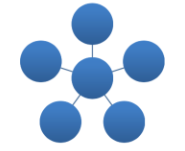
\includegraphics[width=\textwidth]{img/star}
        \caption{\textit{Star Topology}}
        
        \begin{flushleft}
            In the \textbf{Star} topology every peripheral nodes is connected to a central node called \textit{hub} or \textit{switch}. It has an higher cost and complexity than the \textit{bus} topology, but it is much more robust (if the \textit{hub} goes down it is a \textit{single point of failure}).
        \end{flushleft}
        
    \end{minipage}
    \begin{minipage}[t]{0.3\textwidth}
        \centering
        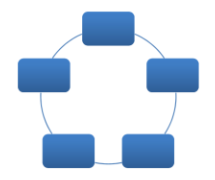
\includegraphics[width=\textwidth]{img/ring}
        \caption{\textit{Ring Topology}}
        
        \begin{flushleft}
            The \textbf{Ring} topology is a \textit{daisy chain} in a closed loop. When a node sends data to another, the data passes through each intermediate node on the ring until reach its destination (it use only one direction). It is not too munch expensive, but has higher complexity (if you want add a new node it could be troublesome).
        \end{flushleft}
        
    \end{minipage}
\end{figure}
In the autonomotive domain it is chosen the \textbf{\textit{Bus Topology}}, why? The first thing is that in the automotive industry it is mandatory to maintain lower the cost. The \textit{busses} are very cheap for the materials, the weight and the volume. In the \textit{bus} topology it is possible to have higher modularity, you can \textit{plug \& play} a node ``when you want'', in that way it is possible to have fully customizability inside the vehicles. The last things is that there is shorter development cycles.
In the autonomotive field there is three main component:
\begin{enumerate}[nosep]
    \item \textbf{\textit{transceiver}}: it is the \textit{physical layer definition} and implement the first layer of the \textit{ISO/OSI} stack.
    \item \textbf{\textit{communication controller}}: it is the communication protocol and implement the first and the second layers of the \textit{ISO/OSI} stack.
    \item \textbf{\textit{ECU}}: also know like \textbf{electronic controller unit} and implement the last layer of the \textit{ISO/OSI} stack, the \textbf{application} layer.
\end{enumerate}
The idea is to made possible to abstract the application layer in order to, if you want, change the first two layers, for example from CANBus to FlexRay, but nothing change at the application layer.

\section{Controller Area Network}
The \textbf{Controller Area Network} also know as \textbf{CAN} is a vehicle bus standard to enable efficient communication. It is originally developed to reduce complexity and cost of electrical wiring. \textbf{\textit{CANBus}} use an \textbf{electrical} medium over wires and a \textbf{broadcast} data transmission. CANBus use the \textbf{\textit{CSMA/CR}} like \textit{multiple access protocol}, it means \textit{carrier sense multiple access collision resolution} protocol, that permit to CANBus to have \textbf{\textit{arbitration}} on the channel access. In this way there is random access to the physical channel, but it is impossible that there is some collision on the communications.
\begin{figure}[h]
    \centering
    \label{img:canbus_1}
    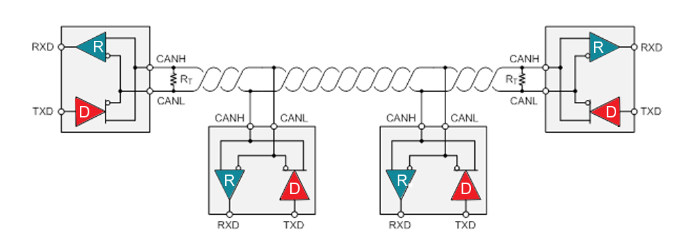
\includegraphics[width=0.75\textwidth]{img/canbus_1}
    \caption{CANBus Network Topology}
\end{figure}

The \textbf{CANBus} network is compose by two wires: \textbf{CAN High} and \textbf{CAN Low}. The data is transmit over the wire using the \textit{potential difference} on each transceiver. Two twisted wires are use because it gives to the protocol \textbf{noise resistance} and \textbf{increase resiliency}, if one brakes, CAN Low \textit{survives}. At the end of the wire in the bus topology there are place two impedance $R_T$ of $120\ohm$. Each CANBus node has three element:
\begin{itemize}[nosep]
    \item \textbf{CAN Transceiver}: is directly connected to the medium access by two pin (one on CANH and the other on CANL). It has the goal to translate the voltage level into bits (during the reception) and send it to the \textit{CAN Controller} and translate bit into voltage level (during the  transmission).
    \item \textbf{CAN Controller}: is connect to the \textit{CAN Transceiver} by two pin (CANTX and CANRX) and is scope is to: message completion, control bus access, transmission and reception of the message, bit timing.
    \item \textbf{Microcontroller}: application software communicating with other ECUs via messages over the bus.
\end{itemize}